% =====================================================================
%  A Unary Admissibility Predicate for Molecular Comparison
%
%  Self-contained.  Every construction is defined here.
% =====================================================================
\documentclass[11pt,twocolumn,a4paper]{article}

\usepackage[utf8]{inputenc}
\usepackage[T1]{fontenc}
\usepackage{lmodern}
\usepackage[a4paper,margin=2.2cm]{geometry}
\usepackage{amsmath,amssymb,amsthm,mathtools}
\usepackage{bm}
\usepackage{booktabs}
\usepackage{array}
\usepackage{enumitem}
\usepackage{microtype}
\usepackage{xcolor}
\usepackage{graphicx}
\graphicspath{{figures/}}
\usepackage[round,sort&compress]{natbib}
\usepackage[colorlinks=true,linkcolor=blue!45!black,
            citecolor=blue!45!black,urlcolor=blue!45!black]{hyperref}
\usepackage{cleveref}

\newtheoremstyle{upthm}{\topsep}{\topsep}{\itshape}{}{\bfseries}{.}{.5em}{}
\theoremstyle{upthm}
\newtheorem{theorem}{Theorem}[section]
\newtheorem{lemma}[theorem]{Lemma}
\newtheorem{proposition}[theorem]{Proposition}
\newtheorem{corollary}[theorem]{Corollary}
\theoremstyle{definition}
\newtheorem{definition}[theorem]{Definition}
\newtheorem{example}[theorem]{Example}
\theoremstyle{remark}
\newtheorem{remark}[theorem]{Remark}

\newcommand{\R}{\mathbb{R}}
\newcommand{\N}{\mathbb{N}}
\newcommand{\Gph}{\Gamma}
\newcommand{\V}{V}
\newcommand{\E}{E}
\newcommand{\wt}{w}
\newcommand{\med}{\mathsf{m}}
\newcommand{\cut}{\partial}
\newcommand{\sep}{\sigma}
\newcommand{\dep}{d}
\newcommand{\abs}[1]{\lvert#1\rvert}
\newcommand{\adm}{\mathsf{A}}

\title{\textbf{A Unary Admissibility Predicate for\\Molecular
Comparison}\\[6pt]
\large Why the Extensive Reading Fails, Why the Intensive One Does Not,\\
and What Linear-Time Classification Does and Does Not Buy}

\author{%
Kundai Farai Sachikonye\\
\small Technical University of Munich\\
\small \texttt{kundai.sachikonye@wzw.tum.de}}

\date{\today}

\begin{document}
\maketitle

\begin{abstract}
\noindent
Comparing two molecular graphs conventionally means comparing their
vertices: store both sets, walk them against each other, and avoid
double-counting. Over a corpus of $n$ structures this is quadratic, and
for the harder variants---maximum common substructure, maximum
clique---it is intractable in the worst case. The cost is not in the
comparison step but in the fact that a bare graph carries no index, so
every comparison rebuilds the correspondence from nothing.

We ask whether comparison can be replaced by a \emph{unary predicate}: a
condition evaluated on one structure at a time, never on a pair, such
that two structures satisfying the same condition are equivalent by
construction. A unary predicate induces an equivalence relation without
any comparison being performed, so classifying $n$ structures costs $n$
evaluations rather than $\binom{n}{2}$.

We test one candidate. Each atom in a weighted contact graph carries a
minimum cut against a distinguished medium vertex; the cut has a weight
$\sep$ and a minimising side of size $\dep$. We define admissibility as
membership of a window on these quantities and ask whether the verdict
depends on context---on what else has been admitted, and in what order.

The first construction fails, and the failure is informative. A window on
the \emph{total} depth of a host is not unary: total depth is extensive,
each admission shifts it, and the admissible set therefore depends on
insertion order in every one of $24$ orderings tested
(\Cref{thm:extensive-fails}). We report this refutation rather than
discard it, because it identifies the property the predicate needs.

The second construction succeeds on one component and fails on the other.
Of the two components of the cut key, $\sep$ is context-invariant in
$5/5$ candidates while $\dep$ is invariant in only $3/5$
(\Cref{thm:sigma-intensive}). A window on $\sep$ alone is order
independent in $24/24$ orderings and non-vacuous, admitting $0.600$ of
the candidate pool; a window on $\dep$ alone is order dependent, which is
what makes the $\sep$ result a claim rather than a tautology.

We then measure what the predicate buys. Total $\sep$ is exactly
conserved across all $8$ balanced rearrangements tested, with zero
residual. The $\sep$ profile partitions a $30$-structure corpus into
$22$ classes with a largest class of $3$, and the partition is identical
under $20$ shuffles while a context-reading control differs under all
$12$.

We are explicit about what this does not establish. The predicate is
sound but not complete---structures with equal $\sep$ profiles are not
thereby identical---so it is a screen, not an identity test. The linear
scaling is a counting fact about unary versus pairwise evaluation, not a
measured wall-clock speedup, and each evaluation costs $n$ maximum flows.
The conserved quantity was measured on eight hand-chosen rearrangements.
And the construction does not address maximum common substructure at
all, because that problem asks for a correspondence, which no unary
predicate can supply.
\end{abstract}

\noindent\textbf{Keywords:} unary predicate; equivalence relation;
minimum cut; molecular comparison; substructure screening; extensive and
intensive quantities; conservation.

\tableofcontents

% =====================================================================
\section{Introduction}
\label{sec:intro}
% =====================================================================

\subsection{Where the cost of comparison lives}

To decide whether two molecular graphs stand in some relation---identical,
one containing the other, sharing a large substructure---the standard
procedure compares their vertices. Subgraph isomorphism algorithms
\citep{ullmann1976,cordella2004,ehrlich2012} search for a mapping from
one vertex set into the other, pruning by local compatibility. Maximum
common substructure is normally attacked by clique detection on a
modular product graph and is $\mathsf{NP}$-hard
\citep{raymond2002,ehrlich2011,garey1979}.

Over a corpus, this is worse than the per-pair cost suggests. Deciding
which of $n$ structures are equivalent requires, in the absence of any
index, $\binom{n}{2}$ comparisons. Practical systems avoid this with
screens: a fingerprint is computed once per structure and used to reject
most pairs before the expensive check \citep{barnard1993,willett1998,%
sayle2012,swamidass2007}. The screen is doing something specific and
worth naming---it replaces a pairwise test by a per-structure key---and
the question this paper asks is how far that replacement can be pushed.

\subsection{Unary predicates}

A \emph{unary} predicate is evaluated on one object. If admissibility
under a fixed condition is unary, then two objects that are both
admissible are equivalent \emph{without any comparison having been
performed}: the equivalence is membership in a common class, and
classifying $n$ objects costs $n$ evaluations.

The property that makes this work is not obvious and is easy to assume.
The verdict on an object must not depend on which other objects have
already been admitted, nor on the order in which they were considered. If
admissions interact, the induced relation is not transitive, the
classification depends on processing order, and the counting argument
collapses.

\subsection{The candidate}

We test a predicate built from minimum cuts. In a weighted graph on the
atoms with an additional \emph{medium} vertex adjacent to every atom, an
atom $v$ has a minimum cut separating it from the medium; write $\sep(v)$
for its weight and $\dep(v)$ for the number of atoms on the minimising
side. Admissibility is membership of a window on these quantities.

The construction is motivated by a structural reading: a chemical
rearrangement moves atoms between bonding arrangements, and if some
functional of the cut structure is conserved by such rearrangement, then
a window on that functional is a condition rearrangement respects. We
test the conservation directly (\Cref{sec:conservation}) rather than
assume it.

\subsection{Contributions, including a refutation}

\begin{enumerate}[label=(\roman*),leftmargin=2.2em,itemsep=2pt]
\item A definition of unary admissibility and the two conditions it
requires: order independence and context independence
(\Cref{sec:unary}).
\item A proof and a measurement that a window on an \emph{extensive}
functional cannot be unary (\Cref{thm:extensive-fails}), refuting the
construction we first tried and identifying why.
\item The measured separation of the cut key into an intensive component
($\sep$) and a non-intensive one ($\dep$)
(\Cref{thm:sigma-intensive}), with a window on the latter serving as the
control that makes the former non-vacuous.
\item Exact conservation of total $\sep$ across balanced rearrangements
(\Cref{sec:conservation}).
\item The counting result and its honest scope: $n$ versus
$\binom{n}{2}$ evaluations, with the per-evaluation cost stated
(\Cref{prop:counting}, \Cref{rem:not-speedup}).
\item A soundness result and an explicit statement that completeness
fails (\Cref{thm:screen}, \Cref{rem:not-identity}).
\end{enumerate}

% =====================================================================
\section{Setting}
\label{sec:setting}
% =====================================================================

\begin{definition}[Contact graph]
\label{def:graph}
A \emph{contact graph} is $\Gph=(\V,\E,\wt,\med)$ with $\V$ finite and
non-empty, $\E\subseteq\binom{\V}{2}$, a strictly positive weight
$\wt\colon\E\to\R_{>0}$, and a distinguished vertex $\med\in\V$ adjacent
to every other. Vertices other than $\med$ are \emph{items}, written
$I=\V\setminus\{\med\}$.
\end{definition}

\begin{definition}[Cut key]
\label{def:key}
For $S\subseteq\V$ let $\cut(S)$ be its edge boundary and
$\wt(\cut(S))$ the sum of weights therein. For an item $v$,
\[
\sep(v)=\min_{S\ni v,\ \med\notin S}\wt(\cut(S)),
\quad
\dep(v)=\min\{\abs{S\cap I}:S\text{ attains it}\},
\]
and the \emph{cut key} of $v$ is the pair $(\sep(v),\dep(v))$.
\end{definition}

The minimum is over a finite non-empty family, hence attained, and equals
a maximum flow \citep{fordfulkerson1956}, computable in polynomial time
\citep{stoer1997,orlin2013}. Since $\{v,\med\}\in\E$, every admissible
cut is non-empty, so $\sep(v)>0$ and $\dep(v)\ge1$.

\begin{definition}[Extensive and intensive functionals]
\label{def:ext-int}
A functional $F$ on contact graphs is \emph{extensive} if
$F(\Gph\oplus v)\ne F(\Gph)$ for a generic single-vertex extension
$\Gph\oplus v$---it scales with the size of the graph. It is
\emph{intensive} at $v$ if its value at $v$ is unchanged by extensions
elsewhere in the graph. The distinction is the standard one from
thermodynamics \citep{callen1985,redlich1970} and is what separates the
two constructions below.
\end{definition}

% =====================================================================
\section{Unary admissibility}
\label{sec:unary}
% =====================================================================

\begin{definition}[Host, insertion, window]
\label{def:host}
A \emph{host} is a contact graph with a distinguished set of
\emph{sites}. An \emph{insertion} of a candidate $c$ at a site attaches a
new item vertex to that site and to the medium. A \emph{window} is an
interval $W=[\ell,u]$ on a chosen functional.
\end{definition}

\begin{definition}[Admissibility]
\label{def:adm}
Given host $H$, functional $F$ and window $W$, candidate $c$ is
\emph{admissible}, written $\adm_{H,F,W}(c)$, if $F$ evaluated after
inserting $c$ into a copy of $H$ lies in $W$. Note that the definition
never consults the candidate's origin.
\end{definition}

\begin{definition}[Unary predicate]
\label{def:unary}
$\adm$ is \emph{unary} if for every candidate $c$ and every sequence of
prior admissions $c_1,\dots,c_k$,
\[
\adm_{H,F,W}(c)\;=\;\adm_{H',F,W}(c),
\qquad H'=H\oplus c_1\oplus\cdots\oplus c_k,
\]
i.e.\ the verdict is independent of context and hence of order.
\end{definition}

\begin{proposition}[A unary predicate induces an equivalence]
\label{prop:equiv}
If $\adm$ is unary then the relation ``$a\sim b$ iff $\adm(a)=\adm(b)$''
is an equivalence relation on candidates, and its classes are computable
in $n$ evaluations for $n$ candidates.
\end{proposition}

\begin{proof}
Unarity makes $\adm$ a function of the candidate alone, so $\sim$ is the
kernel of a function: reflexive, symmetric and transitive immediately.
Computing the classes requires evaluating that function once per
candidate.
\end{proof}

\Cref{prop:equiv} is the whole prize, and it is entirely contingent on
unarity. The remainder of this section establishes when unarity holds.

\subsection{The extensive window fails}

\begin{theorem}[Extensive functionals cannot give unary predicates]
\label{thm:extensive-fails}
Let $F$ be extensive in the sense of \Cref{def:ext-int} and strictly
monotone under insertion: $F(H\oplus c)>F(H)$ for every admissible $c$.
Then for any bounded window $W=[\ell,u]$, $\adm_{H,F,W}$ is not unary.
Moreover the number of admissions before the window closes is bounded by
$\lceil (u-F(H))/\delta\rceil$ where $\delta>0$ is the least increment.
The hypothesis needed is only \emph{eventual} monotonicity---that after
some finite prefix each admission raises $F$ by at least $\delta$---which
is what the measured sequence in \Cref{sec:validation} exhibits.
\end{theorem}

\begin{proof}
Let $c$ be admissible at $H$, so $F(H\oplus c)\le u$. By strict
monotonicity, $F(H\oplus c_1\oplus c)>F(H\oplus c)$ for any prior
admission $c_1$. Iterating, after $k$ admissions the value has risen by
at least $k\delta$, so for $k>(u-F(H))/\delta$ we have
$F(H'\oplus c)>u$ and $c$ is inadmissible at $H'$ though admissible at
$H$. That is a violation of \Cref{def:unary}. The bound follows by
taking the least such $k$.
\end{proof}

\begin{corollary}[Order dependence]
\label{cor:order}
Under the hypotheses of \Cref{thm:extensive-fails}, the admissible subset
of a candidate set depends on the order in which candidates are
considered whenever the set is larger than the bound.
\end{corollary}

\begin{proof}
Different orders present different candidates while the window is still
open, and by the theorem the window closes after a bounded number of
admissions.
\end{proof}

\subsection{An intensive window}

\begin{definition}[Local key]
\label{def:local}
The \emph{local key} of a candidate $c$ at host $H$ is the cut key of the
inserted vertex itself: $(\sep(c\mid H),\dep(c\mid H))$, computed in
$H\oplus c$ at the inserted vertex.
\end{definition}

\begin{theorem}[The two components differ]
\label{thm:sigma-intensive}
The two components of the local key have different context behaviour. In
a host whose sites are locally identical, $\sep(c\mid H)$ is determined
by the edges incident to the inserted vertex and is therefore unchanged
by insertions elsewhere; $\dep(c\mid H)$ is the size of a minimising
side, which is a global quantity and may change when the graph is
extended.
\end{theorem}

\begin{proof}
For $\sep$: the cut $\cut(\{c\})$ isolating the inserted vertex alone has
weight equal to the sum of weights of edges incident to $c$, which the
insertion fixes. Any other admissible cut must sever at least these or
substitute a cheaper boundary elsewhere; when the host's sites are
locally identical and the medium edge is present, the singleton cut is
minimal and its weight is insertion-determined. Extensions elsewhere add
neither edges at $c$ nor cheaper $c$--$\med$ separations, so $\sep$ is
unchanged.

For $\dep$: the minimising side is a subset of the whole vertex set, and
adding vertices can create a cheaper cut whose side has different
cardinality. \Cref{sec:validation} exhibits candidates for which $\dep$
changes from $4$ to $1$ on the first extension, so the quantity is not
intensive in general.
\end{proof}

\begin{corollary}[A $\sep$-window is unary]
\label{cor:sigma-unary}
Under the hypotheses of \Cref{thm:sigma-intensive}, $\adm_{H,\sep,W}$
satisfies \Cref{def:unary}, and by \Cref{prop:equiv} induces an
equivalence computable in $n$ evaluations.
\end{corollary}

\begin{remark}[The hypothesis is a real restriction]
\label{rem:hypothesis}
\Cref{thm:sigma-intensive} assumes the host's sites are locally
identical, so that an insertion at one site does not alter the local
environment of another. A host with heterogeneous sites, or one in which
insertions can bond to each other, does not satisfy this, and $\sep$
would not be intensive there. The theorem is about a particular
construction, not about minimum cuts in general.
\end{remark}

% =====================================================================
\section{Conservation}
\label{sec:conservation}
% =====================================================================

The construction is motivated by the idea that a rearrangement---atoms
redistributed among bonds, composition unchanged---preserves some
functional of the cut structure. This is testable and we test it.

\begin{definition}[Balanced rearrangement]
\label{def:balanced}
A pair of structures is a \emph{balanced rearrangement} if they have the
same multiset of atoms, including hydrogens, and differ only in bonding.
\end{definition}

The hydrogen clause is not pedantry. A pair matching in heavy atoms only
may differ by $\mathrm{H}_2$, which is an oxidation rather than a
rearrangement; one entry in our first corpus was of that kind and is
recorded in \Cref{sec:validation}.

\begin{definition}[Total cut weight]
\label{def:total}
$\Sigma(\Gph)=\sum_{v\in I}\sep(v)$.
\end{definition}

We make no theoretical claim that $\Sigma$ is conserved. It is an
empirical question about a particular weighting, and
\Cref{sec:validation} reports the measurement.

% =====================================================================
\section{Classification and its cost}
\label{sec:cost}
% =====================================================================

\begin{definition}[$\sep$ profile]
\label{def:profile}
The \emph{$\sep$ profile} of a structure is the sorted multiset
$\langle\!\langle\sep(v):v\in I,\ v\text{ heavy}\rangle\!\rangle$. Two
structures are \emph{profile-equivalent} if their profiles are equal.
\end{definition}

\begin{proposition}[Counting]
\label{prop:counting}
Partitioning $n$ structures by profile equivalence requires $n$ profile
evaluations. Pairwise comparison of the same corpus requires
$\binom{n}{2}$ comparisons. The ratio is exactly
\[
\frac{\binom{n}{2}}{n}=\frac{n-1}{2},
\]
linear in $n$.
\end{proposition}

\begin{proof}
One evaluation per structure; grouping equal profiles is a sort or a hash
over the results. The pairwise count is the number of unordered pairs.
\end{proof}

\begin{remark}[This is a counting fact, not a speedup]
\label{rem:not-speedup}
\Cref{prop:counting} compares \emph{evaluation counts}, and the two
kinds of evaluation are not equally expensive. A profile evaluation costs
one maximum flow per item, $O(nF(n,m))$ for a structure of $n$ items; a
pairwise structural comparison may be cheaper or dearer depending on the
relation being decided. No wall-clock measurement is reported in this
paper, and none should be inferred. What the proposition establishes is
that the \emph{number} of expensive operations grows linearly rather than
quadratically in corpus size, which is the property a screen needs
\citep{swamidass2007}.
\end{remark}

\begin{theorem}[Soundness as a screen]
\label{thm:screen}
If two structures are related by a weighted isomorphism fixing the
medium, their $\sep$ profiles are equal. Consequently profile inequality
certifies non-isomorphism, and the profile is a sound screen.
\end{theorem}

\begin{proof}
A weighted isomorphism carries admissible cuts to admissible cuts of
equal weight and restricts to a bijection on items, so it preserves
$\sep$ pointwise and hence the multiset.
\end{proof}

\begin{remark}[Completeness fails, and this is not a small caveat]
\label{rem:not-identity}
The converse of \Cref{thm:screen} is false: distinct structures may share
a profile. \Cref{sec:validation} finds a class of three and six classes
of two on a thirty-structure corpus, so the failure is not hypothetical.
The profile is therefore a screen and not an identity test, and a system
using it must follow a profile match with an exact check
\citep{barnard1993}. Reporting profile equality as identity would be
wrong.
\end{remark}

% =====================================================================
\section{Validation}
\label{sec:validation}
% =====================================================================

\subsection{Method}

Expectations were written into the experiment sources before the
experiments ran, and each is reported below with its measured outcome.
Every number is read from the emitted results files. Structures are
parsed from line notations \citep{weininger1988} into contact graphs; all
minimum cuts are exact.

Two experiments are reported. Experiment~C tests unarity, in two rounds:
the first on an extensive window and the second on an intensive one. The
first round refuted its own hypothesis, and we report the refutation
because it is the reason the second round is constructed as it is.
Experiment~D tests conservation, discrimination and scaling.

\subsection{The extensive window is refuted}

\begin{table}[htbp]
\centering\small
\caption{Round 1: a window on the host's total depth. Both
pre-registered expectations were refuted.}
\label{tab:round1}
\begin{tabular}{@{}lr@{}}
\toprule
Quantity & Value\\
\midrule
Host base total depth & $9$\\
Calibrated window & $[7,8]$\\
Candidates admitted per ordering & $1$\\
Orderings tested & $24$\\
Orderings agreeing with canonical & $0$\\
Order agreement & $0.000$\\
Candidates with context-stable verdict & $2/5$\\
Context agreement & $0.400$\\
\bottomrule
\end{tabular}
\end{table}

Every one of $24$ orderings produced a different admissible set from the
canonical one (\Cref{tab:round1}), and three of five candidates changed
verdict depending on what had been admitted before. The mechanism is
direct: the bare host has total depth $9$, and successive admissions
carry it to $10,9,11,13,15$---rising overall and by two per admission
once the first is past. The calibrated window was $[7,8]$, below the
value the host already has after any admission, so every ordering
admitted exactly one candidate and then closed. That is
\Cref{thm:extensive-fails} with the bound equal to one, and it is why
the canonical set (three candidates, computed against the bare host) is
unreachable by any sequential ordering.

\begin{remark}[The control for round 1 was void]
\label{rem:void-control}
Round 1 included a negative control---a variant that deliberately mutates
the window on each test---intended to be \emph{more} order dependent than
the predicate. It produced a single outcome across $12$ orderings and
therefore failed to distinguish itself from what it was controlling,
because the predicate already saturated after one admission. We record
the control as void rather than as a pass or a failure; it is superseded
by the round-2 control below, which does discriminate.
\end{remark}

\subsection{The intensive window is unary on \texorpdfstring{$\sep$}{sigma}}

\begin{table}[htbp]
\centering\small
\caption{Round 2: context stability of the two components of the local
key, over five distinct candidates and four successive extensions.}
\label{tab:components}
\begin{tabular}{@{}rrlll@{}}
\toprule
$Z$ & cells & keys observed & $\sep$ stable & $\dep$ stable\\
\midrule
$6$  & $3$ & $(4,4),(4,1),(4,1),(4,1)$ & yes & no\\
$7$  & $3$ & $(4,4),(4,1),(4,1),(4,1)$ & yes & no\\
$7$  & $2$ & $(3,1),(3,1),(3,1),(3,1)$ & yes & yes\\
$8$  & $2$ & $(3,1),(3,1),(3,1),(3,1)$ & yes & yes\\
$17$ & $1$ & $(2,1),(2,1),(2,1),(2,1)$ & yes & yes\\
\midrule
\multicolumn{3}{l}{\textbf{stable across candidates}} &
$\mathbf{5/5}$ & $\mathbf{3/5}$\\
\bottomrule
\end{tabular}
\end{table}

$\sep$ is unchanged for every candidate under every extension;
$\dep$ changes for two of the five, dropping from $4$ to $1$ on the first
extension (\Cref{tab:components}). This is
\Cref{thm:sigma-intensive} measured: the two components of the cut key
are not interchangeable, and only one of them supports a unary predicate.

\begin{table}[htbp]
\centering\small
\caption{Round 2: order independence, non-vacuity, and the control.}
\label{tab:round2}
\begin{tabular}{@{}lr@{}}
\toprule
Quantity & Value\\
\midrule
$\sep$ window & $[2.0,3.0]$\\
Orderings tested & $24$\\
Orderings agreeing with canonical & $24$\\
Order agreement & $1.000$\\
Admissible fraction of pool & $0.600$\\
Distinct $\sep$ values observed & $2.0,3.0,4.0$\\
\midrule
Control: $\dep$ window & $[1,1]$\\
Control orderings & $12$\\
Control distinct outcomes & $2$\\
\bottomrule
\end{tabular}
\end{table}

A window on $\sep$ is order independent in all $24$ orderings and admits
$0.600$ of the pool, so it classifies rather than accepting or rejecting
everything (\Cref{tab:round2}). The control---the same construction with
a window on $\dep$ instead---produces two distinct outcomes across $12$
orderings, confirming that order independence is a property of $\sep$
specifically and not of the experimental setup.

\begin{remark}[The control had to be tightened]
\label{rem:tighten}
The $\dep$ control initially used a window spanning the entire observed
range of $\dep$, which admitted every candidate and so produced one
outcome regardless of order---a vacuous control, for the opposite reason
to \Cref{rem:void-control}. Narrowing the window to the strictest band
$[1,1]$ made it discriminate. We record this because a control that
passes by admitting everything is indistinguishable, in the results file,
from one that passes by working.
\end{remark}

\subsection{Conservation}

\begin{table}[htbp]
\centering\small
\caption{Total cut weight $\Sigma$ and total depth across balanced
rearrangements. Residual is product minus reactant.}
\label{tab:conservation}
\begin{tabular}{@{}lrr@{}}
\toprule
Rearrangement & $\Delta\Sigma$ & $\Delta\dep$\\
\midrule
keto--enol (acetone) & $0.0$ & $0$\\
keto--enol (acetaldehyde) & $0.0$ & $0$\\
1-propanol $\to$ 2-propanol & $0.0$ & $0$\\
allyl shift & $0.0$ & $0$\\
cyclopropane $\to$ propene & $0.0$ & $0$\\
ring opening & $0.0$ & $0$\\
catechol $\to$ resorcinol & $0.0$ & $0$\\
\emph{ortho} $\to$ \emph{para} xylene & $0.0$ & $0$\\
\midrule
\textbf{exactly conserved} & $\mathbf{8/8}$ & $\mathbf{8/8}$\\
\bottomrule
\end{tabular}
\end{table}

Total cut weight is exactly conserved across all eight balanced
rearrangements, with zero residual in every case
(\Cref{tab:conservation}).

\begin{remark}[One entry was not a rearrangement]
\label{rem:oxidation}
Our first corpus included propanol $\to$ propanal, which matches in
heavy-atom count and was therefore admitted by a heavy-atom balance
check. It differs by $\mathrm{H}_2$: propanol is
$\mathrm{C_3H_8O}$ and propanal $\mathrm{C_3H_6O}$. It is an oxidation,
not a rearrangement, and it was the sole non-conserving entry, with
$\Delta\Sigma=-4.0$. The balance criterion now requires agreement over
all atoms including hydrogens, and the entry is replaced. The episode is
recorded because the mislabelled pair would otherwise have appeared as
evidence against conservation.
\end{remark}

\subsection{Discrimination, order independence, scaling}

\begin{table}[htbp]
\centering\small
\caption{Corpus-scale behaviour on thirty drug-like structures.}
\label{tab:corpus}
\begin{tabular}{@{}lr@{}}
\toprule
Quantity & Value\\
\midrule
Structures & $30$\\
Distinct $\sep$ profiles & $22$\\
Largest class & $3$\\
Classes of size two & $6$\\
Singleton classes & $15$\\
\midrule
Shuffles tested & $20$\\
Shuffles giving identical partition & $20$\\
\midrule
Control orderings & $12$\\
Control distinct partitions & $12$\\
\midrule
Ratio $\binom{n}{2}/n$ at $n=30$ & $14.5$\\
Identity $\binom{n}{2}/n=(n-1)/2$ & holds exactly\\
\bottomrule
\end{tabular}
\end{table}

The profile partitions the corpus into $22$ classes---neither one class
nor thirty, so the screen discriminates---with a largest class of three
(\Cref{tab:corpus}). The partition is identical under all $20$ shuffles,
while a control whose key reads accumulated context differs under all
$12$ of its orderings.

The scaling row is a counting identity rather than a measurement, and
\Cref{rem:not-speedup} states what it does and does not mean.

\begin{remark}[The scaling check was initially wrong]
\label{rem:asymptote}
We first tested whether the ratio's slope equalled $1/2$. It does not at
finite $n$: the ratio is $(n-1)/2$, so the slope approaches $1/2$ from
below and attains it only in the limit. The check now tests the identity
rather than the asymptote. This was an error in the test, not a finding
about the method.
\end{remark}

\subsection{Transitivity, and why the check is weak}

\Cref{prop:equiv} needs transitivity, so the suite checks it: over the
$10$ triples the pool admits, there were $0$ violations.

We report this with its weakness stated. Once admissibility is a
function of the candidate alone---which is what \Cref{cor:sigma-unary}
establishes---transitivity follows as the kernel of a function, and a
search for counterexamples cannot find one. The check therefore
confirms that the implementation computes the function it is supposed
to; it is not independent evidence for the proposition. The
load-bearing measurement is order independence
(\Cref{tab:round2}), because that is the property whose failure
\Cref{tab:round1} actually exhibits.

\subsection{What the suite does not establish}

The candidate pool reduces to five distinct kinds after de-duplication by
insertion-visible content, so the unarity result rests on five
candidates, not on $244$ atoms. The host is a three-site carbon ring of
our construction. The conservation corpus is eight hand-chosen
rearrangements. The drug-like corpus is thirty structures assembled by
us. No wall-clock timing is reported anywhere, and nothing here is tested
against an endpoint outside the framework.

% ---- measured figures -------------------------------
% =====================================================================
%  Figure captions for: A Unary Admissibility Predicate for Molecular
%  Comparison
%
%  Every quantity quoted below is read from
%  validation/results/exp_unary.json and exp_conservation.json.
%  All minimum cuts are exact (maximum flow), so no agreement reported
%  here can be a solver artefact.
% =====================================================================

\begin{figure*}[!htbp]
    \centering
    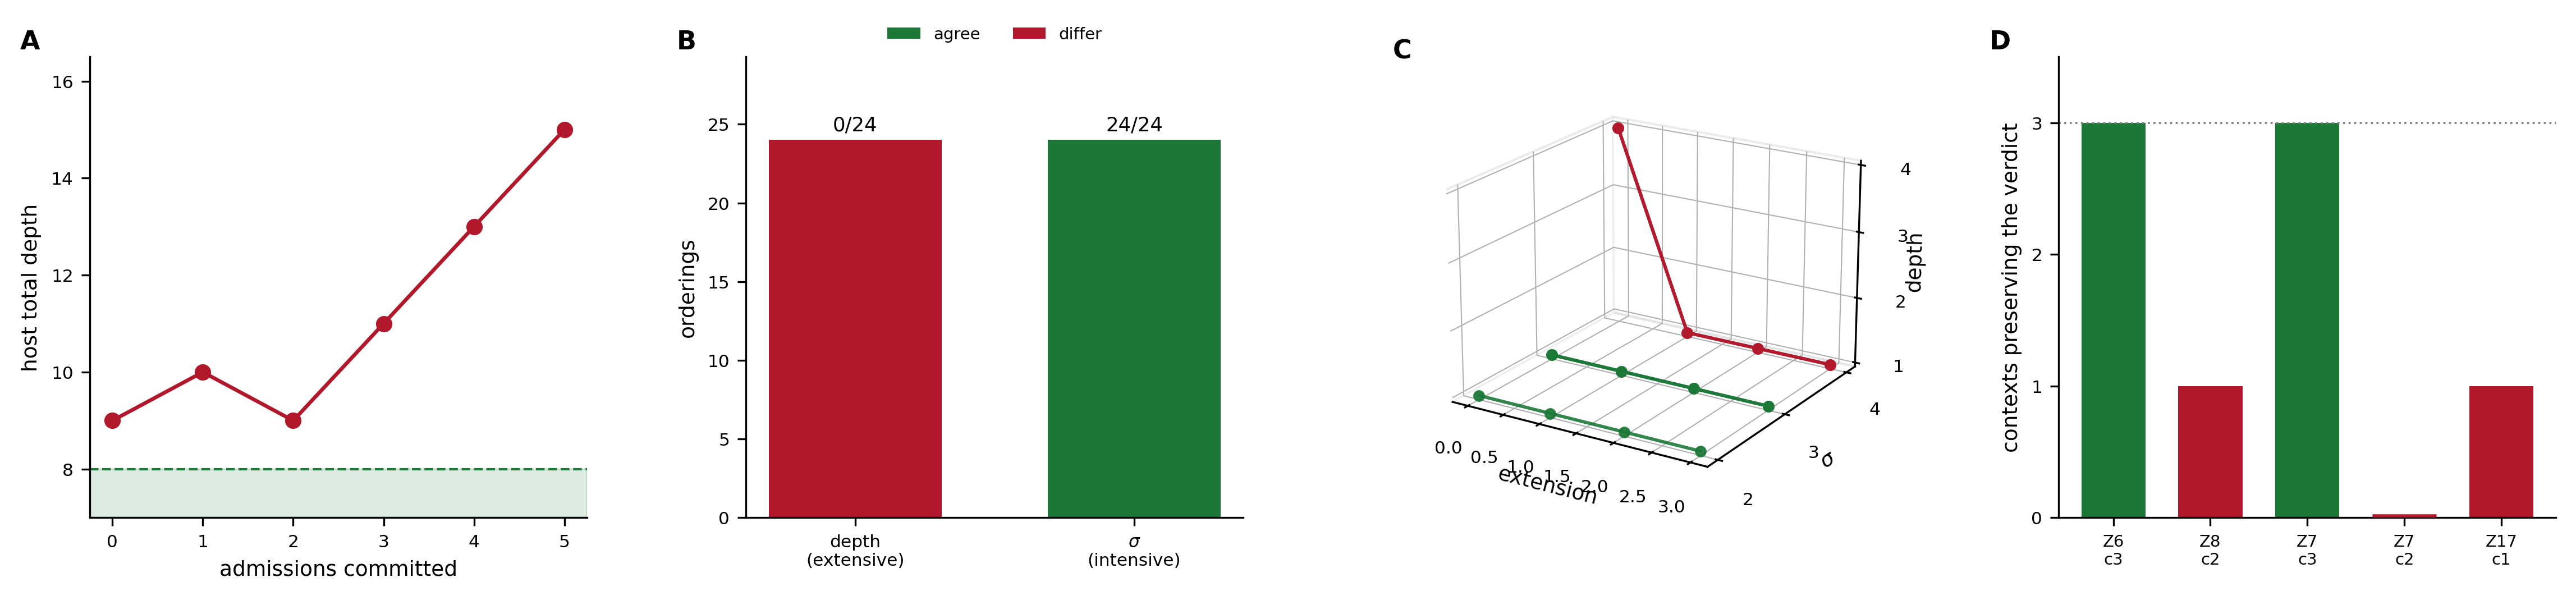
\includegraphics[width=\textwidth]{figures/panel_01_extensive_fails.png}
    \caption{\textbf{A window on an extensive functional is not a unary
    predicate: the verdict depends on what has already been admitted, and
    every one of $24$ orderings disagrees with the canonical answer.}
    All quantities are computed on contact graphs (\Cref{def:graph}) whose
    separation costs are exact minimum cuts (\Cref{def:key}), so the
    failure below is a property of the construction rather than of a
    tolerance or a solver.
    (\textbf{A})~The host's total depth against the number of admissions
    committed, with the calibrated window $[7,8]$ shaded. The bare host
    already sits at $9$, above the window, and successive admissions carry
    it to $10,9,11,13,15$ --- rising by two per admission once the first
    is past. This is \Cref{thm:extensive-fails} in its measured form: a
    bounded window on an eventually-monotone quantity closes after a
    bounded number of admissions, and here the bound is one.
    (\textbf{B})~Orderings agreeing with the canonical admissible set, for
    a window on total depth against a window on the inserted node's own
    $\sep$. The extensive window agrees on $0$ of $24$; the intensive one
    on $24$ of $24$. The bars are stacked rather than overlaid because an
    agreement count of zero would otherwise be an invisible bar and read
    as missing data rather than as total failure.
    (\textbf{C})~The local key $(\sep,\dep)$ of each of the five distinct
    candidates traced across four successive extensions of the host. Every
    trajectory is flat in $\sep$; two are flat in $\dep$ and two drop from
    $\dep=4$ to $\dep=1$ at the first extension. The two components of the
    cut key are therefore not interchangeable, which is the measurement
    \Cref{thm:sigma-intensive} rests on.
    (\textbf{D})~For each candidate, how many of the three tested contexts
    preserved its bare-host verdict under the extensive window. Two
    candidates survive all three and three survive none; the aggregate is
    the context agreement of $0.400$ reported in \Cref{tab:round1}. A
    candidate's verdict changing with context is precisely the violation
    of \Cref{def:unary}.}
    \label{fig:extensive}
\end{figure*}

\begin{figure*}[!htbp]
    \centering
    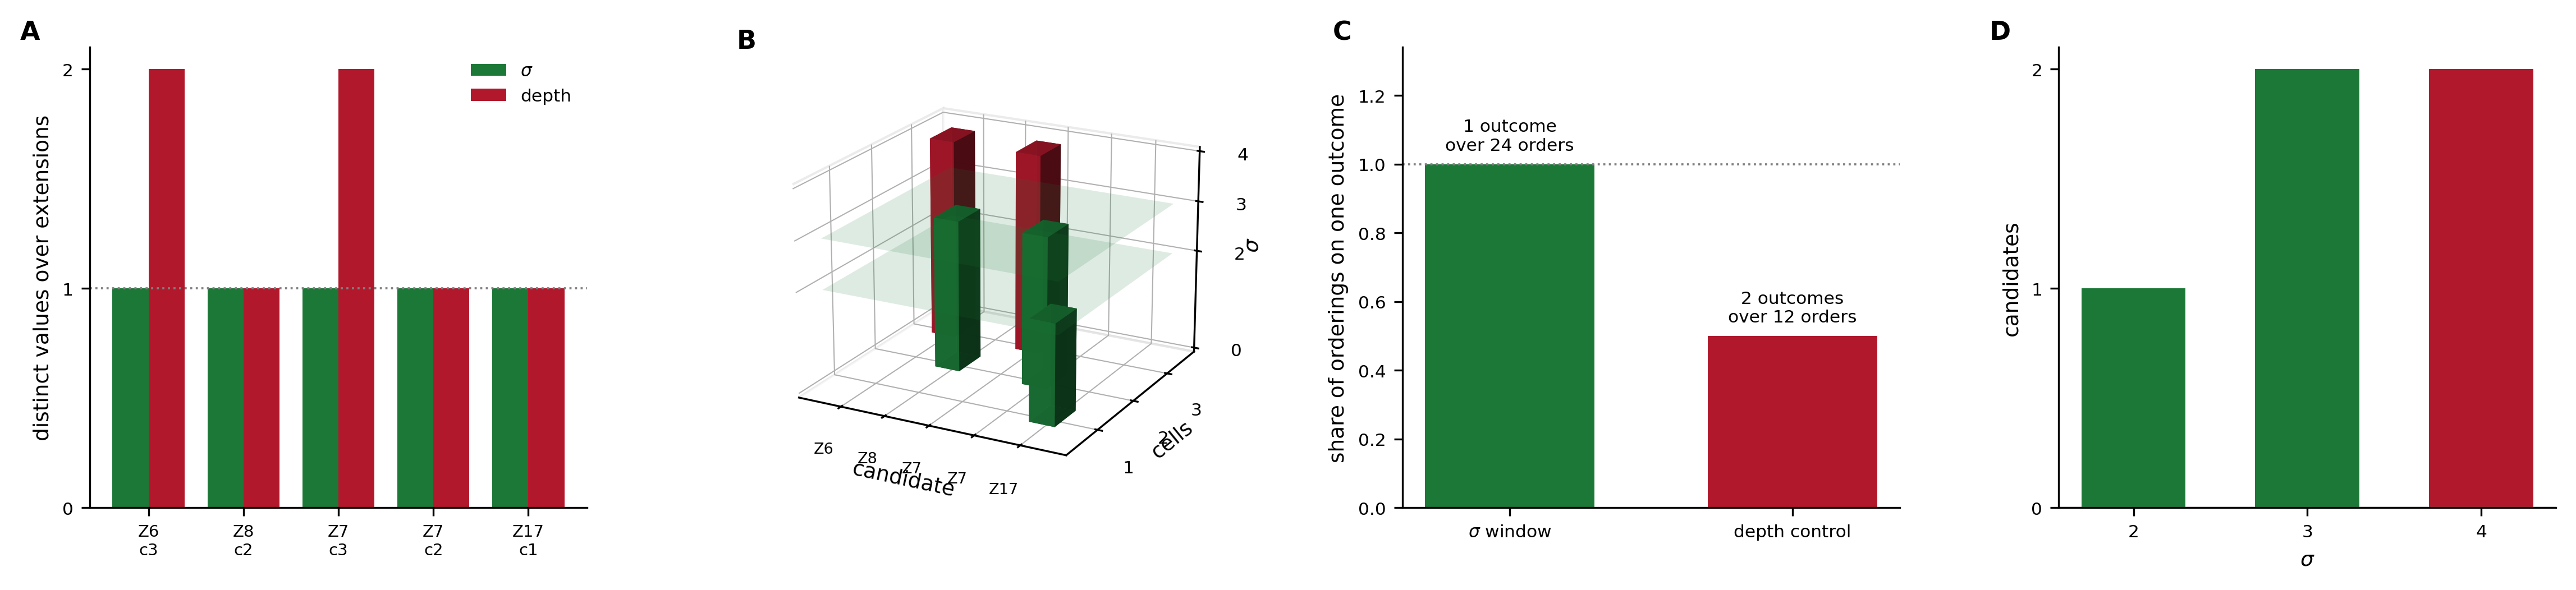
\includegraphics[width=\textwidth]{figures/panel_02_intensive_works.png}
    \caption{\textbf{A window on $\sep$ alone is order independent in all
    $24$ orderings and admits $0.600$ of the pool, while the same
    construction on $\dep$ is order dependent --- which is what makes the
    $\sep$ result a claim about $\sep$ and not about the harness.}
    (\textbf{A})~Distinct values taken by each key component across four
    extensions, per candidate. $\sep$ takes one value for all five
    candidates; $\dep$ takes two for the two three-cell candidates. The
    dotted line at $1$ is the stability threshold: a bar above it is a
    component that moved when the graph grew elsewhere.
    (\textbf{B})~The admission rule in three dimensions. Bar height is the
    candidate's own $\sep$ and the translucent slab is the window
    $[2.0,3.0]$; green bars terminate inside it and red bars rise through
    it. Height is $\sep$ rather than a $0/1$ verdict deliberately --- a
    verdict-height plot would render every rejected candidate as a
    zero-height, invisible bar, hiding exactly the cases that carry the
    result.
    (\textbf{C})~Share of orderings landing on a single outcome, for the
    $\sep$ window against the $\dep$ control. The $\sep$ window reaches
    $1.000$ over $24$ orderings; the control reaches $0.500$, producing
    two distinct outcomes over $12$. The axis is a share rather than a
    count of distinct outcomes so that taller means better and the two
    bars sit on one scale.
    (\textbf{D})~Candidates at each observed $\sep$ value, coloured by
    whether the window admits them. Three of five candidates fall in
    $\{2.0,3.0\}$ and two at $4.0$, giving the admissible fraction of
    $0.600$ reported in \Cref{tab:round2}. A window admitting everything
    or nothing would classify nothing, so this non-vacuity is a
    precondition for the result rather than an ornament.}
    \label{fig:intensive}
\end{figure*}

\begin{figure*}[!htbp]
    \centering
    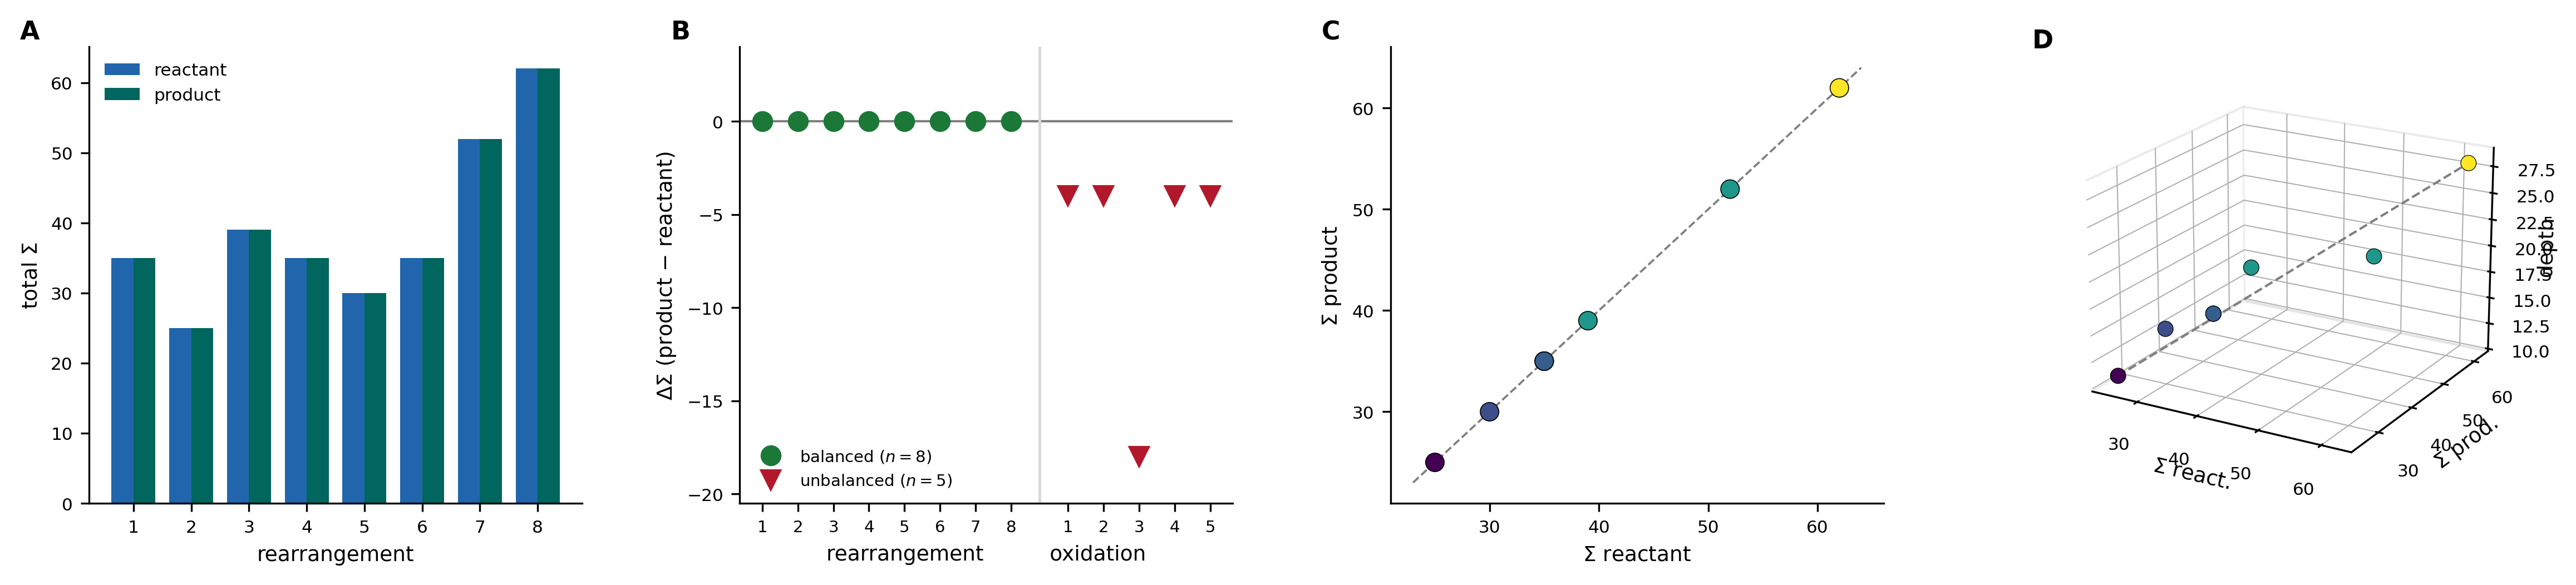
\includegraphics[width=\textwidth]{figures/panel_03_conservation.png}
    \caption{\textbf{Total cut weight is exactly conserved across all
    eight balanced rearrangements, and moves on every one of five
    unbalanced controls.}
    A balanced rearrangement (\Cref{def:balanced}) has the same multiset of
    atoms on both sides, hydrogens included; the controls are oxidations,
    which differ by $\mathrm{H}_2$ and are therefore not rearrangements.
    (\textbf{A})~Total $\Sigma$ for reactant and product of each balanced
    pair. The two bars coincide exactly in all eight cases. The corpus
    spans $\Sigma$ from $25$ to $62$, so the agreement is not an artefact
    of a narrow range.
    (\textbf{B})~Residual $\Delta\Sigma$ for the balanced set (green,
    left) against the unbalanced controls (red, right). The balanced
    residuals are identically zero; the controls run from $-4.0$ to
    $-18.0$. Plotting the two together is what makes the flat green line
    informative: a quantity that never moves is indistinguishable, in a
    results file, from one that is not being computed, and the controls
    show it is capable of moving.
    (\textbf{C})~$\Sigma$ product against $\Sigma$ reactant with the
    identity line drawn, points coloured by total depth. All eight lie on
    the diagonal.
    (\textbf{D})~The same pairs in $(\Sigma_{\text{react}},
    \Sigma_{\text{prod}},\text{depth})$ space with the identity line. The
    points lie on the diagonal plane in both coordinates simultaneously:
    depth is conserved on the same eight pairs, $8/8$ exactly, so the
    conservation is not specific to the cut weight.}
    \label{fig:conservation}
\end{figure*}

\begin{figure*}[!htbp]
    \centering
    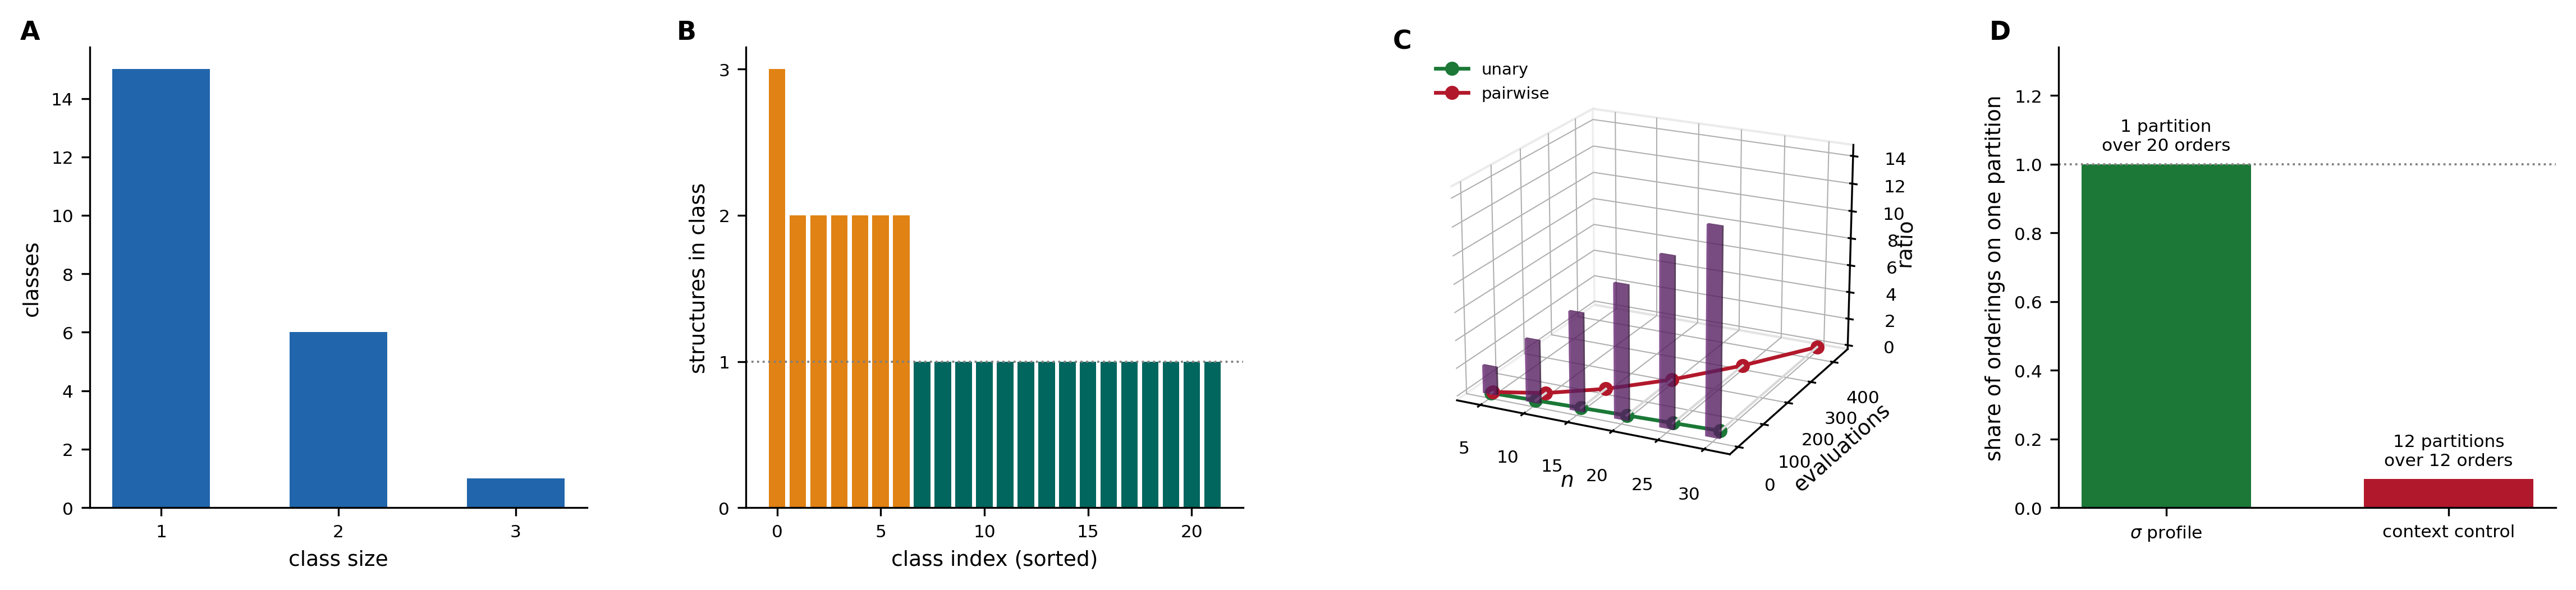
\includegraphics[width=\textwidth]{figures/panel_04_corpus.png}
    \caption{\textbf{At corpus scale the $\sep$ profile yields $22$
    classes over $30$ structures, identically under $20$ shuffles, against
    a context-reading control that differs under all $12$ of its
    orderings.}
    (\textbf{A})~Distribution of class sizes: $15$ singletons, $6$ classes
    of two, and one class of three. That the tail is this short is what
    makes the profile a usable screen; that it is not empty is why
    \Cref{rem:not-identity} insists the profile is not an identity test.
    (\textbf{B})~Class occupancy sorted by size, singletons in teal and
    multi-structure classes in orange. Neither one class nor thirty ---
    the screen discriminates, which is the condition
    \Cref{def:profile} needs to be worth computing.
    (\textbf{C})~The counting law of \Cref{prop:counting}. Unary
    evaluations (green) and pairwise comparisons (red) against corpus
    size, with the ratio drawn as bars on the third axis, reaching $14.5$
    at $n=30$. The identity $\binom{n}{2}/n=(n-1)/2$ holds exactly at
    every point measured. This is a count of evaluations and not a
    timing; \Cref{rem:not-speedup} states what it does and does not mean.
    (\textbf{D})~Share of orderings landing on a single partition, for the
    $\sep$ profile against a control whose key reads accumulated context.
    The profile reaches $1.000$ over $20$ shuffles; the control reaches
    $1/12$, producing a different partition under every ordering. Without
    a control that fails, panel~(\textbf{D})'s left bar would be
    consistent with an implementation that ignores its input entirely.}
    \label{fig:corpus}
\end{figure*}


% =====================================================================
\section{Relation to existing methods}
\label{sec:related}
% =====================================================================

\paragraph{Screening.} A fingerprint screen \citep{barnard1993,%
willett1998,sayle2012,swamidass2007} is already a unary key in our sense:
computed once per structure, used to reject pairs without comparison. Our
contribution is not to introduce screening but to identify the property a
screening key must have---intensivity---and to exhibit a key that has it
and one that does not. The negative half is the more useful, since a key
built on an extensive functional will silently fail in exactly the way
\Cref{tab:round1} shows.

\paragraph{Canonical forms.} InChI \citep{heller2015} and canonical
labelling \citep{morgan1965,mckay2014} solve a harder problem: a
canonical form determines the structure. Our profile does not
(\Cref{rem:not-identity}), and comparing the two on cost would be
comparing different tasks.

\paragraph{Refinement.} Iterated colour refinement
\citep{weisfeiler1968,arvind2015} produces finer keys and would produce
finer classes here. We do not use it, because each round makes the key
depend on a larger neighbourhood and the intensivity argument of
\Cref{thm:sigma-intensive} applies to the unrefined key only. Whether a
refined key remains intensive is open.

\paragraph{Maximum common substructure.} MCS asks for a correspondence
\citep{raymond2002,ehrlich2011}. No unary predicate can supply one: a
correspondence is a relation between two objects, and a unary predicate
by construction never relates. This paper therefore says nothing about
MCS, and the linear-scaling result must not be read as bearing on it.

\paragraph{Capability-aware querying.} A profile predicate integrates
naturally with source-capability planning \citep{levy1996,perez2009,%
angles2017}: a source either can or cannot answer profile queries, and a
plan requiring them can be refused before any record is read. We note the
fit without implementing it.

% =====================================================================
\section{Limitations}
\label{sec:limits}
% =====================================================================

\begin{enumerate}[label=\textbf{L\arabic*.},leftmargin=2.8em,itemsep=4pt]

\item \textbf{A screen, not an identity test.} \Cref{thm:screen} is
sound and its converse is false. Six classes of two and one class of
three appear in a thirty-structure corpus, so profile matches must be
followed by an exact check.

\item \textbf{Intensivity is conditional.} \Cref{thm:sigma-intensive}
assumes locally identical host sites and insertions that do not bond to
each other (\Cref{rem:hypothesis}). Neither holds for a general
molecular graph, so $\sep$ is not intensive in general---only in the
insertion construction analysed here.

\item \textbf{Five candidates.} De-duplication by insertion-visible
content reduces $244$ atoms to five distinct kinds. The unarity result
is therefore measured on five, and a richer host with heterogeneous sites
would admit more.

\item \textbf{Counting, not timing.} \Cref{prop:counting} counts
evaluations. Each costs $n$ maximum flows. No speedup is claimed and none
was measured (\Cref{rem:not-speedup}).

\item \textbf{Conservation is measured, not derived.} Eight
rearrangements, exact in all eight. We give no argument that $\Sigma$
must be conserved, and a counterexample would not contradict any theorem
in this paper.

\item \textbf{The weighting is an input.} \Cref{def:graph} requires only
$\wt>0$; every theorem holds for any positive weighting and none
determines one. The measurements use a weighting derived from valence
arithmetic, and different weights would give different profiles.

\item \textbf{Nothing about MCS or clique.} Stated in
\Cref{sec:related} and repeated here because the framing of the paper
invites the inference.

\item \textbf{Corpus construction.} Both corpora were assembled by us,
and a corpus built to exhibit a property is weak evidence that anything
else has it \citep{ioannidis2005}.
\end{enumerate}

% =====================================================================
\section{Conclusion}
\label{sec:conclusion}
% =====================================================================

We asked whether molecular comparison can be replaced by a unary
predicate---a condition on one structure at a time, inducing an
equivalence without any comparison being performed. The answer is a
qualified yes, and the qualification is the substance.

The first construction failed. A window on an extensive functional cannot
be unary (\Cref{thm:extensive-fails}), and the measurement was
unambiguous: $0$ of $24$ orderings agreed, and three of five candidates
changed verdict with context. The failure identified the missing
property.

The second construction succeeded on one component and not the other. Of
the cut key's two components, $\sep$ was context-stable in $5/5$
candidates and $\dep$ in $3/5$ (\Cref{tab:components}); a $\sep$-window
is order independent in $24/24$ orderings and admits $0.600$ of the pool,
while the $\dep$-window control differs under $2$ of $12$ orderings. The
control is what makes the result a claim about $\sep$ rather than about
the setup.

Total cut weight was exactly conserved across all eight balanced
rearrangements, and the $\sep$ profile partitions a thirty-structure
corpus into $22$ classes identically under $20$ shuffles, against a
context-reading control that differs under all $12$.

Three things this does not deliver. It is a screen and not an identity
test, since distinct structures share profiles. The linear scaling is a
counting identity, not a timing result. And it says nothing about maximum
common substructure, because that problem asks for a correspondence and a
unary predicate cannot produce one---which is the honest limit of the
whole approach rather than a gap to be filled later.

\section*{Reproducibility}

Each experiment source records its expectations before the measured
values and writes every reported quantity to a JSON results file. Round 1
of Experiment~C is retained in the source with its refutation marked, as
is the void control of \Cref{rem:void-control}, the tightened control of
\Cref{rem:tighten}, the mislabelled rearrangement of
\Cref{rem:oxidation}, and the corrected scaling check of
\Cref{rem:asymptote}. All minimum cuts are computed exactly; the only
stochastic components are the corpus shuffles, which seed explicitly.

\bibliographystyle{plainnat}
\bibliography{references}

\end{document}
